% Draft: replace author placeholders before submission. No invented team metadata.
\documentclass[10pt,twocolumn,letterpaper]{article}
\usepackage[pagenumbers]{cvpr}
\usepackage[T1]{fontenc}
\usepackage{microtype}
\usepackage[hidelinks]{hyperref}
\graphicspath{{figures/}}
\newcommand{\todo}[1]{\textcolor{red}{[TODO: #1]}}
\title{Clinical-Trial Stopping Reasons and Outcomes:\\Semi-Supervised Prediction and Calibrated Classification}
\author{\todo{Part 1 contributor: full name} \and \todo{Part 2 contributor: full name}\\
CS5785 / ORIE5750 / ECE5414, Cornell University, Fall 2026}
\begin{document}
\maketitle
\noindent\textbf{Responsibilities.} Part 1 contributor: reason-label preprocessing,
semi-supervised recovery, classifier experiments and predictions. Part 2 contributor:
outcome modeling, calibration and reason-based error analysis.
\todo{Confirm full names, responsibilities and any additional team members.}

\begin{abstract}
We study stopping-reason prediction and trial-outcome classification using
semi-supervised learning and calibrated classification. For five overlapping stopping reasons, a K-Means/3-neighbor
hybrid followed by weighted logistic regression achieves validation sample F1
0.88675 and macro F1 0.77923. For trial success, pooled eligibility-text TF-IDF
logistic regression with phase encoding achieves validation log loss 0.57375;
training-only, trial-grouped sigmoid calibration modestly improves it to 0.57221.
Predicted reasons enable recorded-reason coverage in the outcome error analysis. Probability metrics improve modestly, while some small
reason groups retain high false-success rates. Temporal shift, predicted-reason
error and repeated validation selection limit generalization claims.
\end{abstract}

\section{Methods}
\subsection{Data and leakage controls}
We use only the supplied assignment data~\cite{assignment}. Part 1 has 1,171
training trials (157 visible labels; 1,014 rows masked as $-100$), 78 validation
trials and 312 test trials. Reasons are Safety, Funding, Efficacy, Recruitment
and Other; several may apply. Labeled trials start earlier on average than unlabeled trials (2001.72 versus 2006.42), so observed label priors may not represent the masked population. Part 2 has 8,037/1,013/1,500 train/validation/test
phase rows. Validation phases I/II/III have 149/501/363 rows; test has 500 each.
Repeated combined-phase trials stay within one supplied split. IDs match records
but are never predictive features. No deep learning or external outcome labels
are used.

Neither outcome training nor calibration uses reason labels, embeddings,
predictions, or their derived groups.

\subsection{Part 1: recovery and classification}
Standardize the 150 reason embeddings on all training rows. Fit K-Means with
$K\in\{5,10,20\}$, k-means++ initialization, 10 starts, tolerance $10^{-4}$,
300 iterations and seed 42. Compare diagonal GMMs with three starts, tolerance
$10^{-3}$, 200 iterations and covariance regularization $10^{-5}$.
For hard/soft membership $r_{ik}$ and observed reason prior $\pi_j$, estimate
\begin{equation}
q_{kj}=\frac{\sum_{i\in L}r_{ik}y_{ij}+2\pi_j}{\sum_{i\in L}r_{ik}+2}.
\end{equation}
Threshold the recovered scores at 0.3 or 0.5; if none crosses, assign the
highest-scoring reason. Preserve all observed labels. Fit five L2 logistic
regressions (liblinear, at most 1,000 iterations, seed 42) with $C\in\{0.1,1\}$
and pseudo-row weight 0.25 or 1. Observed rows have weight 1. Final decisions
use 0.5 with the same nonempty fallback.

The 70-setting initial suite includes supervised controls, 48 cluster-augmented
settings, and added-year/text ablations with $C\in\{0.1,1,10\}$. Text/drug TF-IDF
uses minimum frequency 3, up to 3,000 unigrams and sublinear term frequency;
all transformations fit training only. PCA is diagnostic, not clustering input.
Four Funding-only threshold controls (0.30/0.20/0.15/0.10) hold the other reasons
fixed. Twenty-five local-recovery controls compare direct K-NN, K-NN recovery,
and cluster/local hybrid recovery with $K\in\{3,5,9,15\}$ and uniform/distance
voting, plus matched supervised LR. This gives 99 evaluated configurations.

The selected hybrid equally averages scores from the best 10-cluster model
and three uniform neighbors among the 157 labeled training trials. Recover
masked labels at 0.3 with the fallback, then fit LR with $C=0.1$ and pseudo-weight
0.25. Select by validation sample F1, then macro F1. K-Means/GMM and feature
construction use standard scikit-learn implementations~\cite{clustering,tfidf}.

\subsection{Part 2: fixed model and controlled experiments}
First predict each phase's training success prior. Compare 36 LR settings:
three text sets (criteria; diseases/drugs/ICD; all four), $C=0.1/1/10$, year
on/off, and pooled versus independent phase models. Safely parse list-valued
text; missing text becomes empty. Each field has training-fitted unigram/bigram
TF-IDF with minimum frequency 3, sublinear TF, L2 normalization, at most 15,000
criteria features or 5,000 per other field. Pooled models include one-hot phase;
per-phase models fit independent transforms. Year uses training-median imputation,
missingness indicators and scaling. LR uses liblinear, tolerance $10^{-5}$,
at most 2,000 iterations and seed 5785, without class weights.

Select minimum overall validation log loss without a validation refit. The winner
uses criteria plus phase, pooled $C=1$, no year. Overall validation loss is
row-weighted; report equal-phase mean separately because test phases are balanced.
F1 uses probability $\geq0.5$; ROC-AUC and average precision (AP) use success
probabilities. AP is not trapezoidal PR area.

\subsection{Training-only probability calibration}
Generate exactly one out-of-fold margin for every training row using five
shuffled StratifiedGroupKFold folds, grouping by trial ID and approximately
balancing phase/outcome strata (seed 5785). Each fold refits the same TF-IDF,
phase encoding and $C=1$ LR on its fit rows. Fit an unpenalized two-parameter
sigmoid to these OOF margins/labels, either pooled or independently by phase.
The calibrator never sees validation labels. At inference, transform margins
from the original full-training base model; this is not a fold ensemble.
OOF models see roughly 80\% of training rows, so a margin-distribution mismatch
with the full base remains possible. Sigmoid calibration follows the standard
probability-calibration formulation~\cite{calibration}.

\subsection{Reason-based outcome error analysis}
For outcome failures only ($y=0$), join Part 2 trial\_id to Part 1 ID. Use visible
train/validation reasons first. Otherwise use the final hybrid's saved masked-train
pseudo-labels or test predictions. Absent Part 1 records form a distinct
no-record group; masked/prediction-unavailable rows are not negative reasons.
A multi-label trial contributes to every positive reason, once within each phase.
For each phase/group compute count, false-success count/fraction and mean success
probability, retaining truth/prediction provenance. Compare the same group
membership before/after calibration. Empty groups have undefined rates.

\section{Results}
\subsection{Part 1}
\begin{table}[t]
\centering\small
\input{part1_results}
\caption{Initial Part 1 validation F1 by reason and method.}
\label{tab:p1}
\end{table}
The initial cluster methods underperform supervised controls
(Table~\ref{tab:p1}). Added year/text features do not improve initial augmented
models (Table~\ref{tab:p1features}); this does not establish that all text or chemistry features are unhelpful. Funding's maximum smoothed cluster score is 0.2051, below 0.3; lowering
its threshold adds 112 pseudo-positives but drops sample F1 from 0.8547 to
0.8419 through false positives because an entire mixed cluster is promoted. The hybrid instead recovers 16 Funding positives
and identifies 2/4 Funding validation positives without false positives. It wins
sample F1 0.88675; K-NN-only recovery has higher macro F1 0.78730. The recorded
hybrid public Kaggle F1 is 0.87927~\cite{artifacts}; it is a leaderboard score,
not a fully labeled test evaluation. No fitted Part 1 model file is saved, but
recovered labels, validation/test predictions and source are available.

\begin{table}[t]
\centering\small
\input{part1_feature_results}
\caption{Sample F1 by feature set: embeddings (E), year (Y), and text (T).}
\label{tab:p1features}
\end{table}
\begin{table}[t]
\centering\small
\input{part1_knn_results}
\caption{Local recovery validation F1 by reason and method.}
\label{tab:p1knn}
\end{table}

\begin{figure}[t]
\centering\includegraphics[width=\linewidth]{part1_pca_clusters.pdf}
\caption{Existing training-only PCA diagnostic for Part 1; the first two PCs
retain only 24.2\% of embedding variance. Source: final Part 1 notebook.}
\label{fig:pca}
\end{figure}

\subsection{Part 2 probability and phase metrics}
The phase prior has validation loss 0.67199. The best criteria model reaches
0.57375, versus 0.60076 for the best disease/drug/ICD-only setting and 0.58635
for all text. Larger $C$ reduces training loss but worsens validation loss;
the winner's training loss is 0.46903. Adding year does not beat it.
Pooled calibration improves overall loss by only 0.00154 and wins this targeted
comparison (Table~\ref{tab:overall}). Phase-specific calibration improves Phase III
more but worsens Phase I and overall loss relative to pooled calibration
(Table~\ref{tab:phases}). Positive sigmoid slopes preserve within-phase rankings,
so ROC-AUC/AP remain unchanged; the fixed-threshold F1 can move.
\begin{table}[t]
\centering\small\begin{tabular}{lrrrr}
\toprule
Model & Loss & F1 & ROC & AP \\
\midrule
Phase prior & 0.67199 & 0.60578 & 0.59247 & 0.61200 \\
Raw criteria & 0.57356 & 0.74769 & 0.76890 & 0.80485 \\
Selected four-field & 0.56412 & 0.75000 & 0.77854 & 0.82248 \\
\bottomrule
\end{tabular}

\caption{Part 2 validation. Raw: original model; Pool/Phase: pooled or phase-specific
sigmoid. Phase mean weights all phases equally.}
\label{tab:overall}
\end{table}
\begin{table}[t]
\centering\small\setlength{\tabcolsep}{3pt}\begin{tabular}{lrrrrr}
\toprule
Phase & $n$ & Loss & F1 & ROC & AP \\
\midrule
I & 149 & 0.57648 & 0.75145 & 0.75809 & 0.81184 \\
II & 501 & 0.59013 & 0.65944 & 0.74989 & 0.74267 \\
III & 363 & 0.52314 & 0.82657 & 0.79234 & 0.88504 \\
\bottomrule
\end{tabular}

\caption{Validation metrics, F1 at 0.5. ROC denotes ROC-AUC.}
\label{tab:phases}
\end{table}

Phase III is not broadly overconfident: raw mean success probability is 66.05\%
versus 66.12\% observed. Among 79 predictions at least 0.8, mean probability is
85.80\% versus 92.41\% observed success, indicating underconfidence there.
The 0.4--0.5 bin overpredicts (45.21\% versus 26.47\%, $n=34$), so calibration
is mixed (Figure~\ref{fig:reliability}). Pooled Brier improves from 0.19547 to
0.19493 overall and 0.18089 to 0.18019 in Phase III. No leaderboard score is recorded for the selected calibrated model: \todo{add a verified score and submission identity if available}.
\begin{figure}[t]
\centering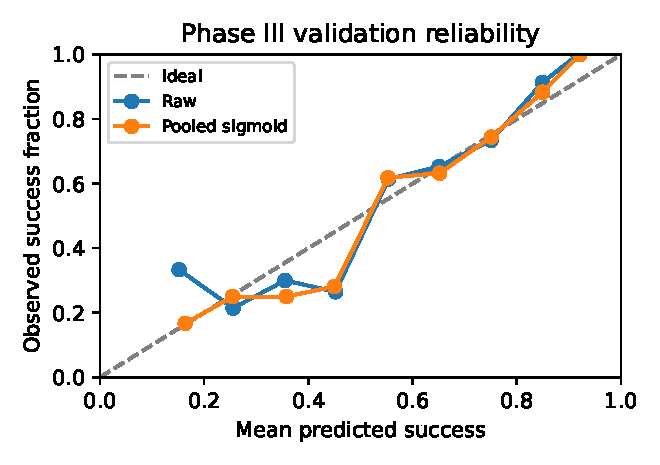
\includegraphics[width=.95\linewidth]{phase3_reliability.pdf}
\caption{Phase III reliability from fixed ten-bin validation summaries. Sparse
bins are noisy; the diagonal denotes perfect calibration. Source: build\_tables.py.}
\label{fig:reliability}
\end{figure}

\subsection{Reason coverage and errors}
Hybrid pseudo-labels are available for 131 phase rows (113 unique trials)
whose reasons were masked; these labels remain estimates. Among 452 unsuccessful phase rows
(398 trials), 27 use true reasons, 171 predicted reasons and 254 have no Part 1
record. Reason estimates are available for all matched records.
\begin{table}[t]
\centering\small\setlength{\tabcolsep}{3pt}\begin{tabular}{llrrrrr}
\toprule
Phase & Reason & $n$ & T & P & False+ & Rate \\
\midrule
I & Safety & 8 & 1 & 7 & 4 & 0.500 \\
I & Funding & 3 & 1 & 2 & 1 & 0.333 \\
I & Efficacy & 4 & 0 & 4 & 4 & 1.000 \\
I & Recruitment & 24 & 2 & 22 & 5 & 0.208 \\
I & Other & 3 & 0 & 3 & 1 & 0.333 \\
I & No record & 28 & 0 & 0 & 11 & 0.393 \\
II & Safety & 11 & 1 & 10 & 4 & 0.364 \\
II & Funding & 4 & 1 & 3 & 0 & 0.000 \\
II & Efficacy & 15 & 0 & 15 & 6 & 0.400 \\
II & Recruitment & 93 & 12 & 81 & 18 & 0.194 \\
II & Other & 15 & 3 & 12 & 5 & 0.333 \\
II & No record & 144 & 0 & 0 & 45 & 0.312 \\
III & Safety & 5 & 1 & 4 & 1 & 0.200 \\
III & Funding & 0 & 0 & 0 & 0 & -- \\
III & Efficacy & 8 & 0 & 8 & 8 & 1.000 \\
III & Recruitment & 25 & 5 & 20 & 16 & 0.640 \\
III & Other & 9 & 2 & 7 & 7 & 0.778 \\
III & No record & 82 & 0 & 0 & 50 & 0.610 \\
\bottomrule
\end{tabular}

\caption{Unsuccessful-trial groups. T/P: true/predicted reason counts;
Raw/Pool: false-success fractions before/after pooled calibration. No record
counts are absent records, not T/P. Groups overlap; -- means undefined.}
\label{tab:reasons}
\end{table}
Phase II Recruitment improves from 18/93 false successes to 15/93, and Phase III
no record from 53/82 to 52/82. Phase III Efficacy stays 7/8, all with predicted
reasons; Phase I Efficacy stays 3/4. These small reason groups do not support
strong rankings or causal explanations. The complete audit also retains mean
predicted probabilities and the phase-specific calibration comparison.

\section{Discussion}
\paragraph{Complementary but separate tasks.}
Coarse cluster averages can suppress rare reasons or promote entire mixed
clusters. Local neighbors provide more specific evidence; their equal blend
with the unsupervised component helped sample F1 here. Quarter-weight pseudo-labels
limit but do not remove labeling errors. PCA cannot establish high-dimensional
separation, and extra sparse text/drug knowledge may add noise with only 157
trusted labels. The final hybrid's 99-setting selection and only four Funding
validation positives limit certainty.

Outcome calibration changes probabilities rather than vocabulary or rankings.
Its small loss gain is not evidence of statistical significance. A high
false-success fraction among failures alone does not establish overconfidence;
calibration must consider all validation outcomes. The reason audit exposes
persistent subgroup errors despite improved aggregate loss. Coverage is complete
for recorded Part 1 trials, but most matched reason labels are estimates;
misclassification and overlapping groups can distort comparisons. No-record
trials may include completed failures, not merely trials with missing explanations.

\paragraph{Temporal and selection limitations.}
Observed train/validation start years end in 2013; test years are 2014--2021.
Training has 21 missing years, validation six. Historical vocabulary, treatment
mix and success rates may change. Random-by-trial validation does not measure
later-year performance; the retained model has no recorded leaderboard result
with which to quantify that gap. Reusing validation for 37 outcome settings and
two calibrators creates selection optimism. Seven training/validation eligibility
texts match exactly, despite disjoint IDs, which may also make validation easier.
Combined-phase rows are correlated, and per-phase sample sizes differ. We report
row and phase-macro losses distinctly. A temporal holdout and repeated-seed checks
are future work, not completed experiments.

\begin{thebibliography}{9}
\bibitem{assignment} Cornell CS5785 / ORIE5750 / ECE5414 course staff.
\emph{Midterm Project}, Fall 2026. Local assignment transcription
\texttt{Midterm\_Project.tex}; PDF unavailable in this checkout.
\bibitem{artifacts} Team project artifacts, Fall 2026.
\texttt{PART1\_NOTES.md}, hybrid selection/prediction files and validation tables.

\bibitem{clustering} Scikit-learn developers. \emph{Clustering}, documentation.
\url{https://scikit-learn.org/stable/modules/clustering.html}.
\bibitem{tfidf} Scikit-learn developers. \emph{TfidfVectorizer}, API documentation.
\url{https://scikit-learn.org/stable/modules/generated/sklearn.feature_extraction.text.TfidfVectorizer.html}.
\bibitem{calibration} Scikit-learn developers. \emph{Probability calibration}, documentation.
\url{https://scikit-learn.org/stable/modules/calibration.html}.
\end{thebibliography}
\noindent\textbf{AI assistance disclosure (review before submission).}
Codex assisted with implementation, verification and drafting.
\todo{Confirm wording against the course policy and each contributor's actual use.}
\end{document}
